% =============================================================================
% File:  XCS.tex -- 
% Author(s): Valentin Plugaru (valentin.plugaru@uni.lu)
% Time-stamp: <Tue 2015-06-16 09:22 svarrette>
% 
% Copyright (c) 2015 Valentin Plugaru<Sebastien.Varrette@uni.lu>
% 
% For more information:
% - LaTeX: http://www.latex-project.org/
% - Beamer: https://bitbucket.org/rivanvx/beamer/
% - LaTeX symbol list:
% http://www.ctan.org/tex-archive/info/symbols/comprehensive/symbols-a4.pdf
% =============================================================================

\documentclass{beamer}
% \documentclass[draft]{beamer}
\usepackage{_style}
\usepackage{setspace}

% The key part to use my theme -- if you precise nothing, the image that
% illustrate the slides is assumed to be images/slides_image.jpg
\usetheme[image=images/logo_ULHPC.pdf]{Falkor}

% Not integrated in my theme as not everybody wants that
\AtBeginSection[]
{
  \frame{
    \frametitle{Summary}
    {\scriptsize\tableofcontents[currentsection]}
  }
}

\graphicspath{{images/}} % Add this directory to the searched paths for graphics

%%%%%%%%%% Header %%%%%%%%%%%%
\title{Extreme Computing Studio (XCS) Portal}
\subtitle{Interactive \& graphical sessions}

\author{Valentin Plugaru}
\institute[PCOG Research unit]{
  Parallel Computing and Optimization Group (\href{http://pcog.uni.lu}{PCOG}),
  University of Luxembourg (\href{http://www.uni.lu}{UL}), Luxembourg
}

% Mandatory to **declare** a logo to be placed on the bottom right -- normally the
% university logo. ADAPT ACCORDINGLY:
\pgfdeclareimage[height=0.8cm]{logo}{images/logo_UL.pdf}

\date{}

%%%%%%%%%%%%% Body %%%%%%%%%%%%%%%
\begin{document}

\begin{frame}
  \vspace{2.5em}
  \titlepage
\end{frame}

% ......
\frame{
  \frametitle{Summary}
  {\scriptsize
    \tableofcontents
  }
}

% ======================== 
%\input{_content.md} % Markdown content
% ======================== 

\section{Graphical sessions}

\frame{
  \frametitle{Using graphical interfaces on UL HPC}
  \center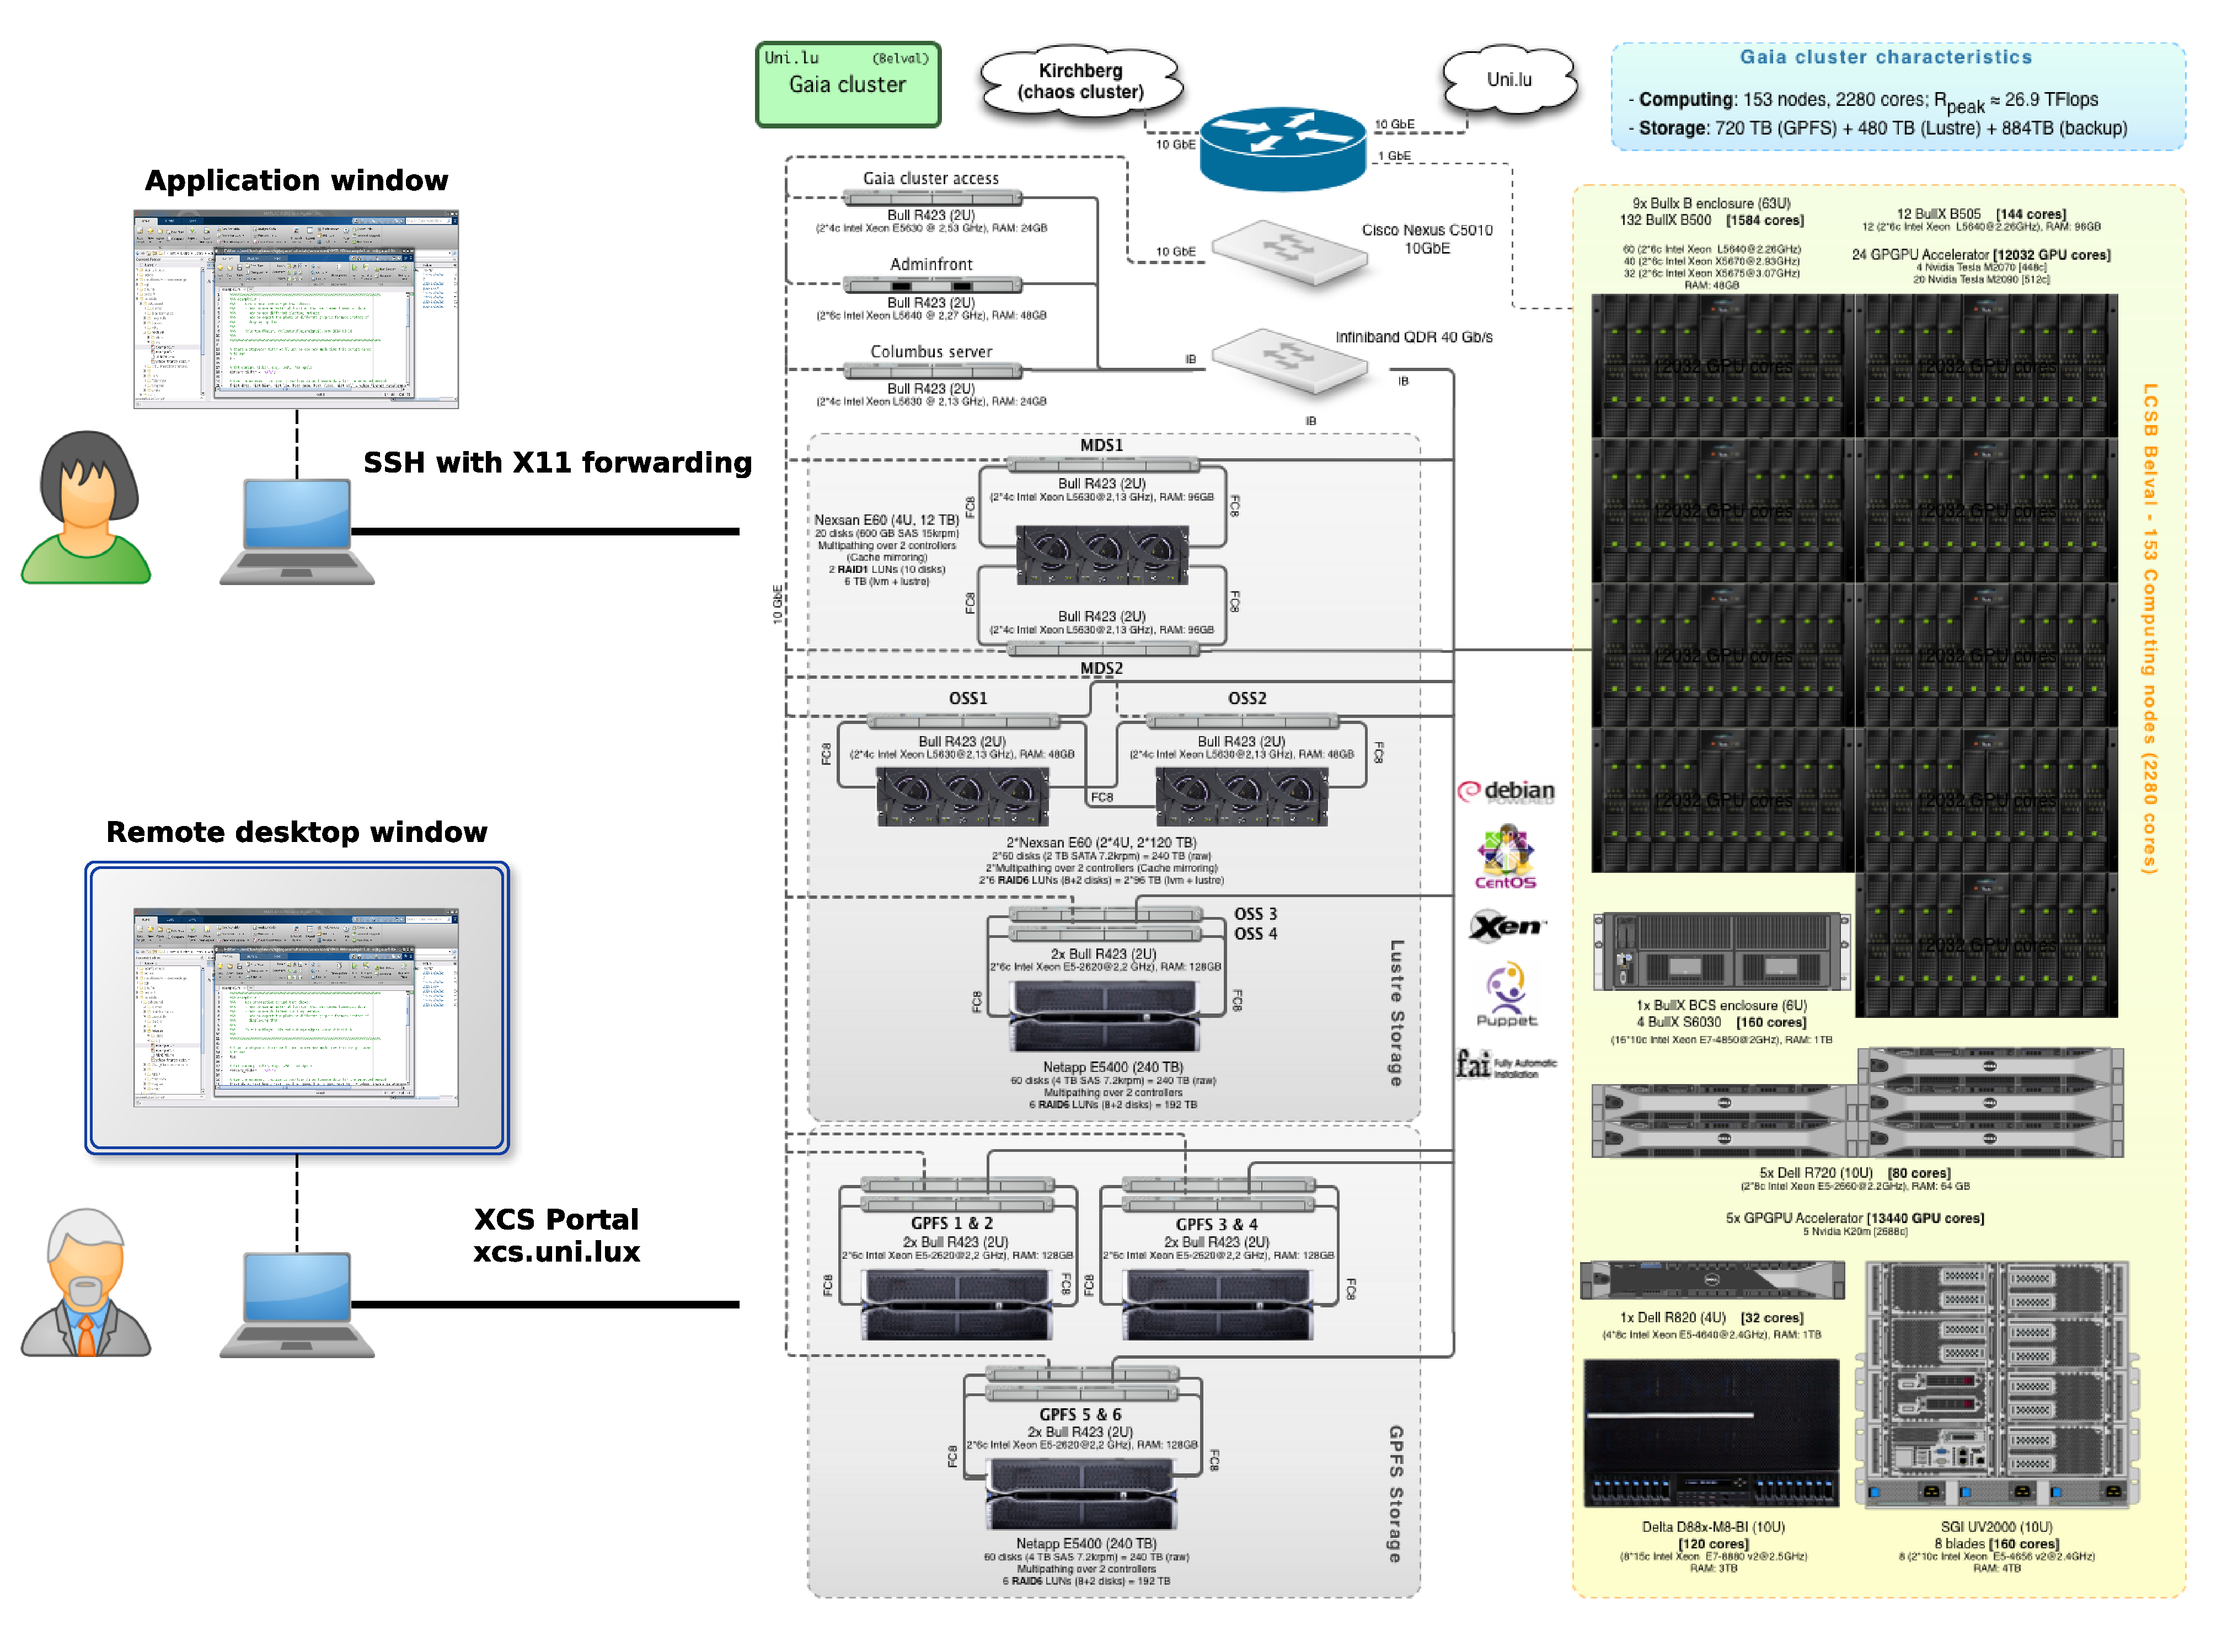
\includegraphics[width=0.85\textwidth]{graphical_sessions}
}

\frame{
  \frametitle{X11 forwarding}
  \begin{itemize}

  \item On Windows 
   \begin{itemize}
    \item \textbf{Putty}: Category $\rightarrow$ Connection $\rightarrow$ SSH $\rightarrow$ X11 $\rightarrow$ Enable X11 forwarding (\textit{check})
    \item \href{http://sourceforge.net/projects/vcxsrv/}{VcXsrv}: Windows X-server, to render locally the remote application
   \end{itemize}
   
   \pause
   \item On OS X
   \begin{itemize}
    \item \textbf{ssh} (in Terminal): use \texttt{ssh -X ...}
    \item \href{http://xquartz.macosforge.org/landing/}{XQuartz}: X Window System libraries and applications, required on some OS X versions
   \end{itemize}

   \pause
   \item On Linux
   \begin{itemize}
    \item \textbf{ssh} (in a console): simply use \texttt{ssh -X ...}
   \end{itemize}
  \end{itemize}
  
  \pause
  \vspace{-4pt}
  \begin{alertblock}{Downsides}
    \begin{itemize}
      \setlength\itemsep{0pt}
      \vspace{-4pt}
      \item Network connection interrupted $\rightarrow$ session crashes
      \item Rendering \emph{slow} (no 3D acceleration) and \emph{network intensive}
      \vspace{-4pt}
    \end{itemize}
  \end{alertblock}

}


\section{The XCS Portal}


\frame{
  \frametitle{Overview}
  \begin{itemize}
   \item Web portal for launching/monitoring visualisation sessions: \href{https://xcs.uni.lux}{xcs.uni.lux}
   \itemhook available from inside the UL network and externally through UL VPN
  \end{itemize}
}

\frame{
  \frametitle{Prerequisites}
  \begin{enumerate}
   \item UL HPC account, you need your \emph{password} to login on \href{https://xcs.uni.lux}{xcs.uni.lux}
   \item your account to be in the XCS group (for now, added on request)
   \item \href{http://sourceforge.net/projects/turbovnc}{TurboVNC}: Virtual Network Computing application tuned for maximum performance and compression with 3D applications
  \end{enumerate}
}

\begin{frame}
  \frametitle{Current applications integrated in XCS}
  \begin{spacing}{0.8}
  \begin{itemize}
    \setlength\itemsep{0pt}
    \onslide<1,5>{
    \item MATLAB 
    \itemhook {\tiny High-level technical computing language and interactive environment for algorithm development, data visualization, data analysis, and numerical computation.}
    \item RStudio 
    \itemhook {\tiny IDE for R, a programming language for statistical computing and graphics.}
  }
  \onslide<2,5>{
    \item SAS (Statistical Analysis System) 
    \itemhook {\tiny Advanced analytics, business intelligence, data management, and predictive analytics software.}
    \item STATA 
    \itemhook {\tiny Complete, integrated statistical software package for data analysis, data management, and graphics.}
  }
  \onslide<3,5>{
    \item ABAQUS 
    \itemhook {\tiny Finite Element Analysis software for modeling, visualization and best-in-class implicit and explicit dynamics FEA.}
  }
  \onslide<4,5>{
    \item VMD 
    \itemhook {\tiny Molecular visualization program for displaying, animating, and analyzing large biomolecular systems using 3-D graphics and built-in scripting.}
    \item ParaView 
    \itemhook {\tiny Data analysis and visualization application.}
  }
  \end{itemize}
  \end{spacing}
\end{frame}



\frame{
  \frametitle{Intro page}
  \center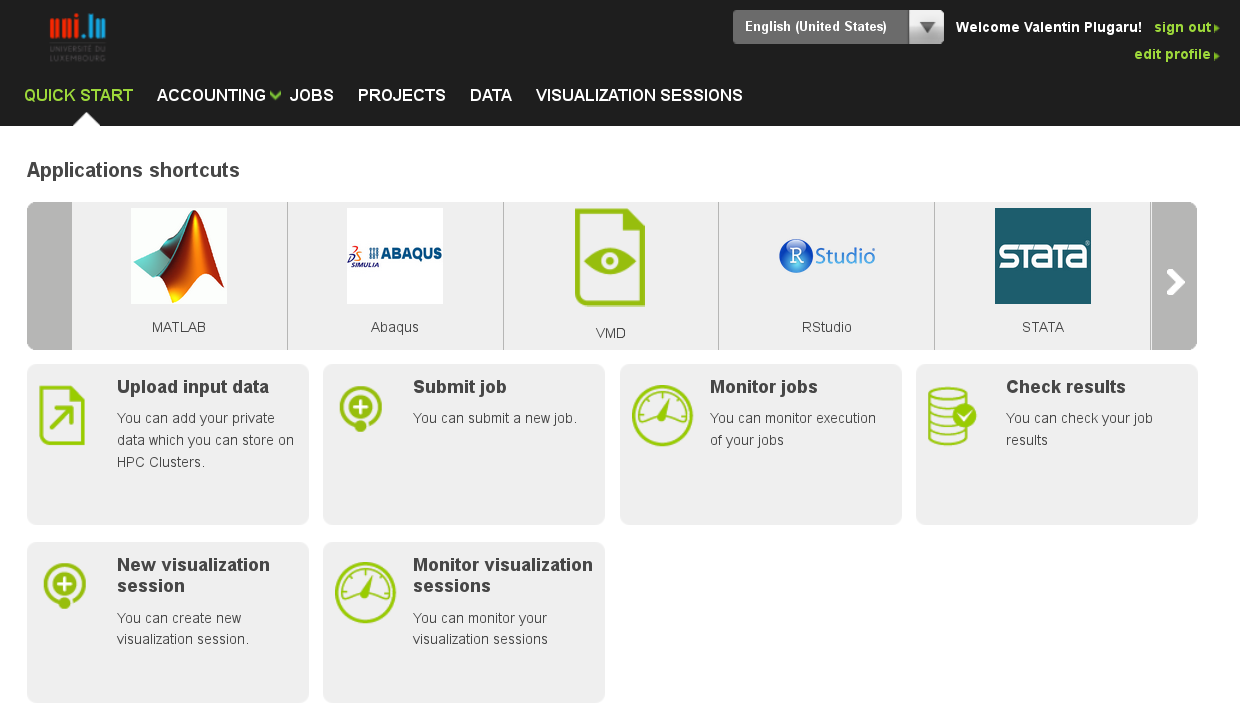
\includegraphics[width=0.85\textwidth]{xcs_quickstart}
}

\frame{
  \frametitle{Launching a graphical session}
  \center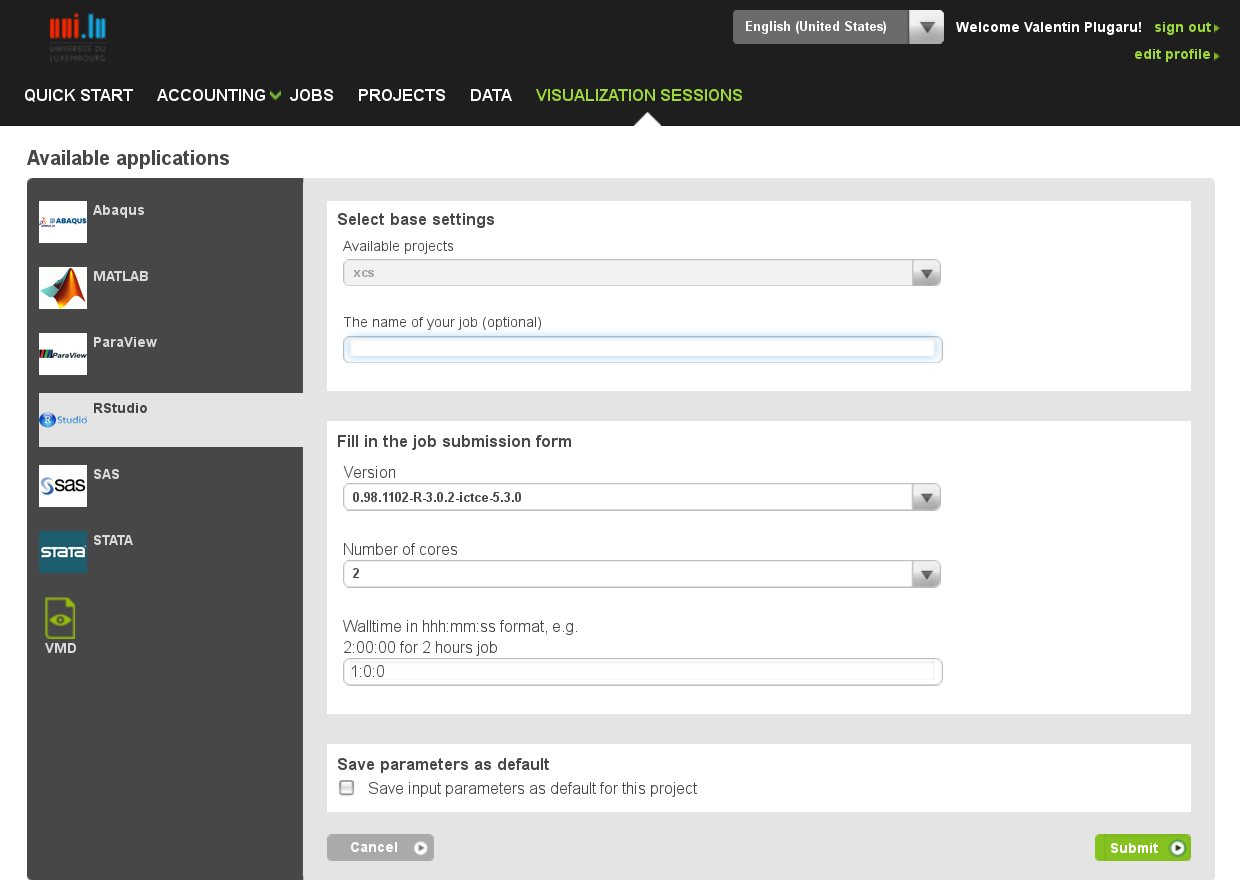
\includegraphics[width=0.85\textwidth]{xcs_launch}
}

\frame{
  \frametitle{Checking job status}
  \center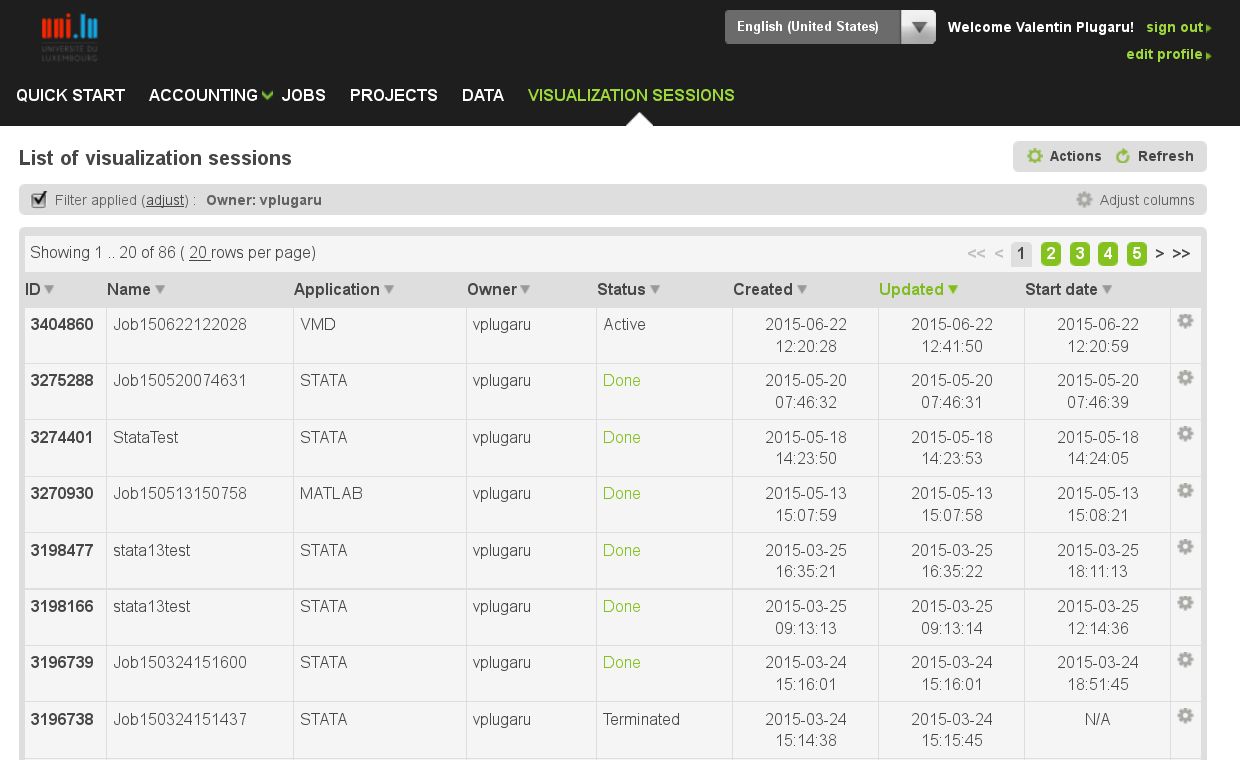
\includegraphics[width=0.85\textwidth]{xcs_jobs}
}

\frame{
  \frametitle{Connecting to a running session}
  \center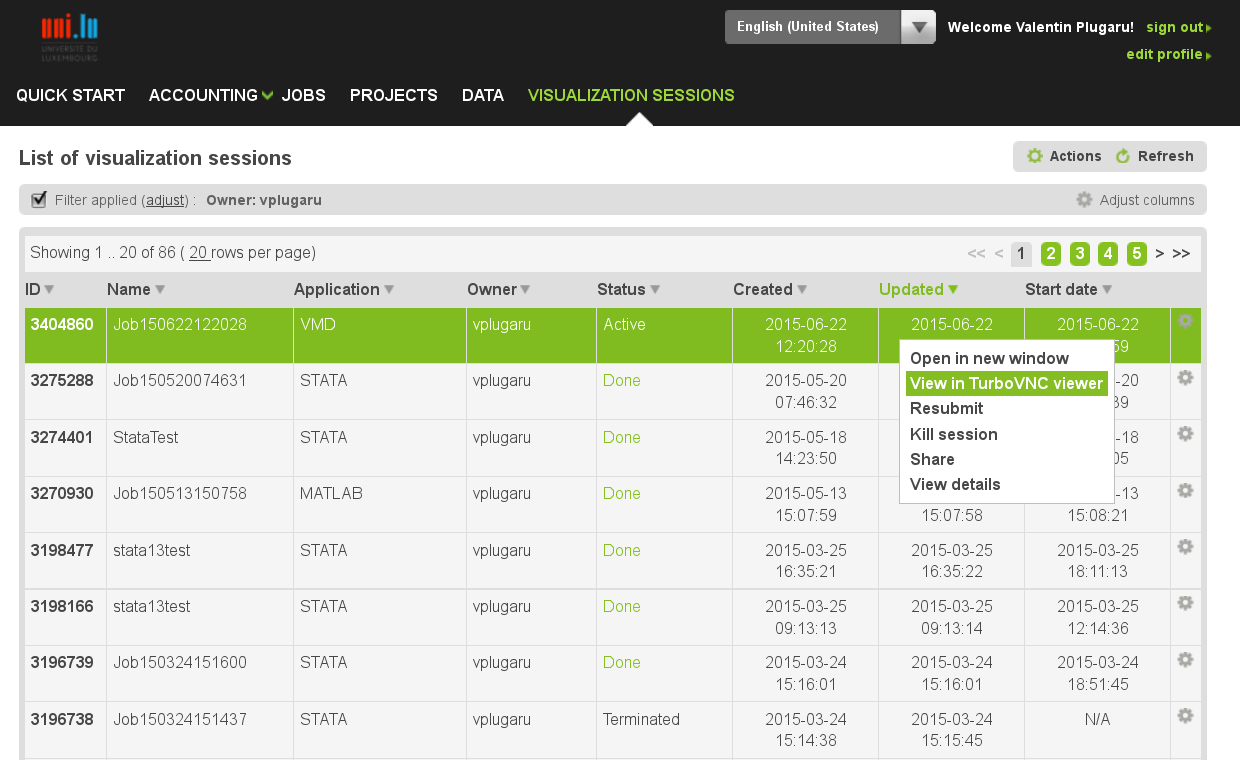
\includegraphics[width=0.85\textwidth]{xcs_connect}
}

\frame{
  \frametitle{Uploading data}
  \center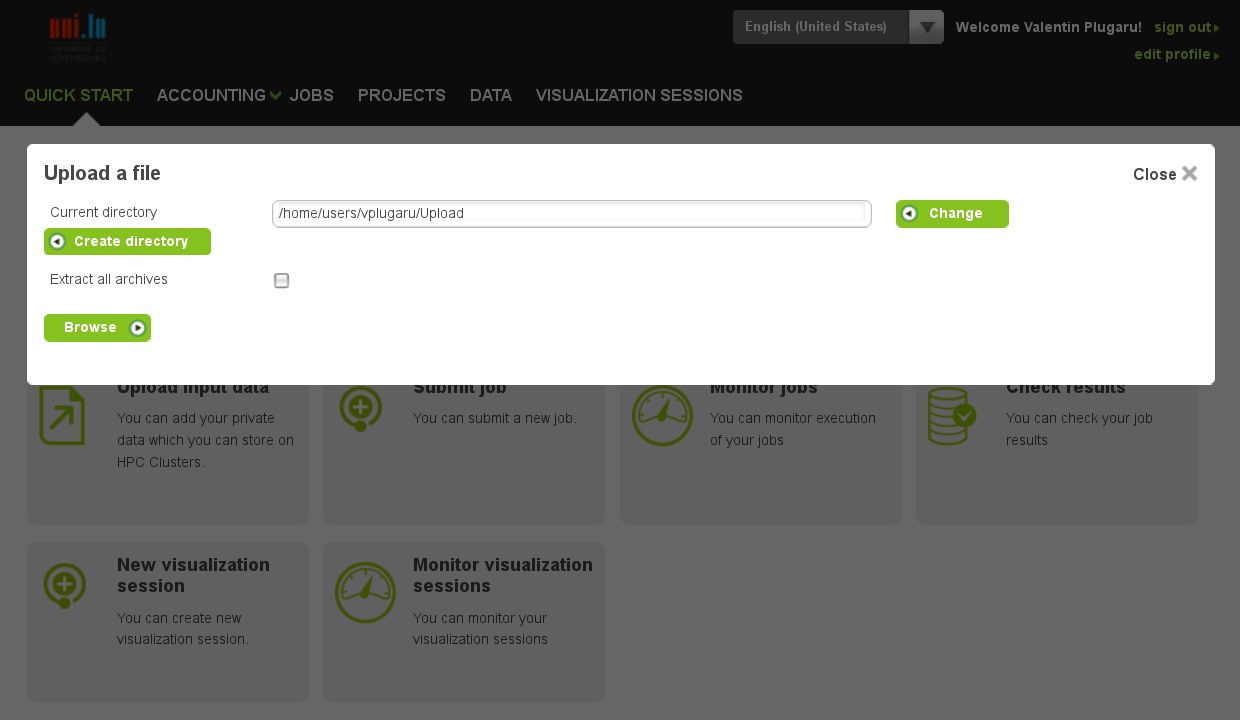
\includegraphics[width=0.85\textwidth]{xcs_upload}
}


% ======================== END =========================
\section*{Thank you for your attention...}
\frame{
  \frametitle{Questions?}
  % ~~~~~~~~~~~~~~
  \begin{columns}
    \column{0.5\textwidth}
    % \emph{Contact}\\
    {\tiny
      \emph{Valentin Plugaru}\\
      ~~~~ \textit{Mail:} \href{mailto:valentin.plugaru@uni.lu}{valentin.plugaru@uni.lu}\\
      ~~~~ Office E-005\\
      ~~~~ Campus Kirchberg\\
      ~~~~ 6, rue Coudenhove-Kalergi\\
      ~~~~ L-1359 Luxembourg

    }
    \column{0.5\textwidth}
    % \scalebox{8}{\emph{?}}
    
\includegraphics[width=1.5in]{question.jpg}
  \end{columns}
  % Below is the table of content over 2 columns
  \vfill
  \begin{multicols}{2}
    {\tiny \tableofcontents}
  \end{multicols}

}

\newcounter{finalframe}
\setcounter{finalframe}{\value{framenumber}}

% %.......
% \frame{
%   \frametitle{}
%   \vfill
%   \centering \LARGE Appendix\footnote{notice the slide number below...}
%   \vfill
% }

\setcounter{framenumber}{\value{finalframe}}

\end{document}

% ~~~~~~~~~~~~~~~~~~~~~~~~~~~~~~~~~~~~~~~~~~~~~~~~~~~~~~~~~~~~~~~~
% eof
% 
% Local Variables:
% mode: latex
% mode: flyspell
% mode: visual-line
% TeX-master: "XCS.tex"
% End:
